我们在第5章中讨论了C++程序的生命周期,由五个主要阶段组成——编写、编译、链接、加载和执行。在正确编译所有源代码之后,需要将它们放到一个可执行文件中。编译过程中产生的目标文件不能由处理器直接执行,这是为什么呢?

为了回答这个问题,就来看看编译器如何用ELF格式(类Unix系统和许多其他系统使用)构造对象文件的:

\begin{center}
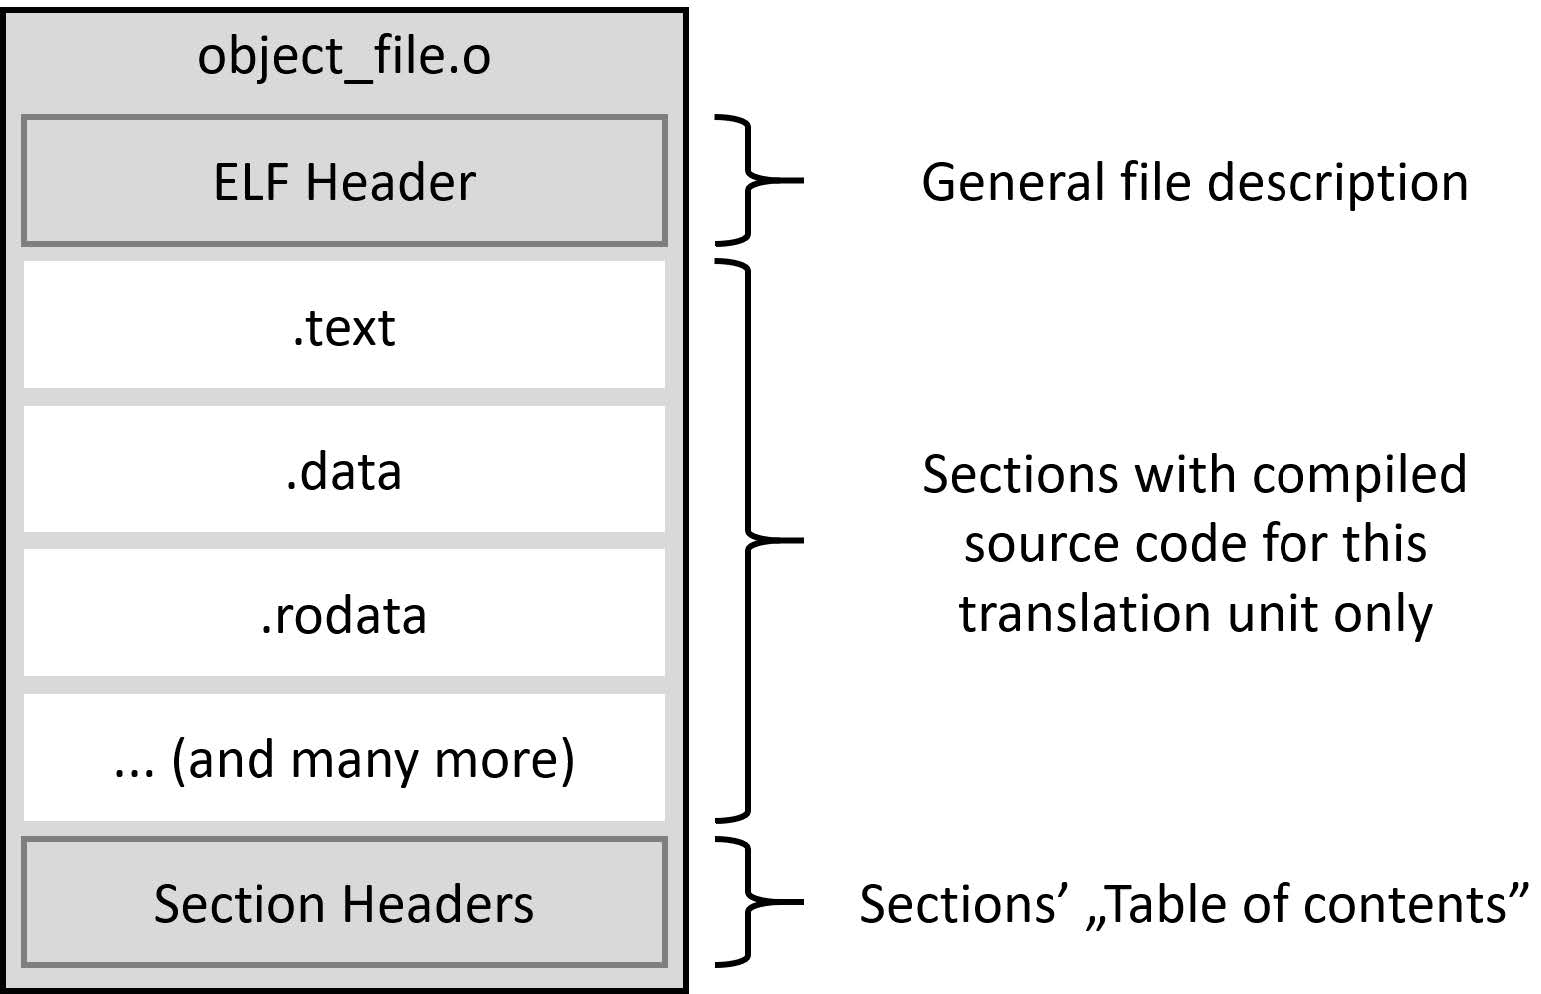
\includegraphics[width=0.8\textwidth]{content/2/chapter6/images/1.jpg}\\
图6.1 目标文件的结构
\end{center}

编译器将为每个翻译单元(为每个.cpp文件)准备一个目标文件。这些文件将用于构建程序的内存映像。Object文件包含以下元素:

\begin{itemize}
\item 
ELF头标识目标操作系统、ELF文件类型、目标指令集体系结构,以及ELF文件中两个头表的位置和大小信息——程序头表(不存在于目标文件中)和节头表。

\item 
包含按类型分组的信息的部分(下面将介绍)。

\item 
节头表,包含关于名称、类型、标志、内存中的目标地址、文件中的偏移量和其他杂项信息,用于了解文件中的哪些部分,以及它们在哪里,就像目录一样。
\end{itemize}

当编译器处理源代码时,将收集到的信息分组到几个单独的格中,这些格将放在属于它们自己的区段中。其中一些如下:

\begin{itemize}
\item 
.text区段:机器代码,包含处理器要执行的所有指令

\item 
.data区段:初始化的全局对象和静态对象(变量)的所有值

\item 
.bss区段:未初始化的全局对象和静态对象(变量)的所有值,这些值将在程序启动时初始化为零

\item 
.rodata区段:常量的所有值(只读数据)

\item 
.strtab区段: 一个字符串表,包含所有常量字符串,例如hello.cpp示例中的Hello World

\item 
.shstrtab区段: 包含所有部分名称的字符串表
\end{itemize}

这些区段非常类似于可执行文件的最终版本,其将放入RAM中以运行我们的应用程序,但不能直接将这个文件加载到内存中。因为每个目标文件都有自己的一组区段。若只是把它们连在一起,就会遇到各种各样的问题。将浪费大量的空间和时间,因为需要更多的RAM页,指令和数据将很难复制到CPU缓存中。整个系统必须要复杂得多,并且会浪费宝贵的CPU周期,在运行时跳过许多(可能是数万个).text、.data和其他部分。

我们要做的是把对象文件的每个部分,和所有其他对象文件中相同类型的部分放在一起。这个过程称为重定位(这就是ELF文件类型为目标文件重定位的原因)。除了将适当的部分组合在一起之外,还必须更新文件中的内部关联——即变量、函数、符号表索引或字符串表索引的地址。所有这些值都是对象文件的本地值,其编号从0开始。将文件捆绑在一起时,需要偏移这些值,使它们指向组合文件中的正确地址。

图6.2显示了重新定位的过程——重新定位.text,从所有链接的文件构建.data,然后是.rodata和.strtab(为了简单起见,图中不包含头文件):

\begin{center}
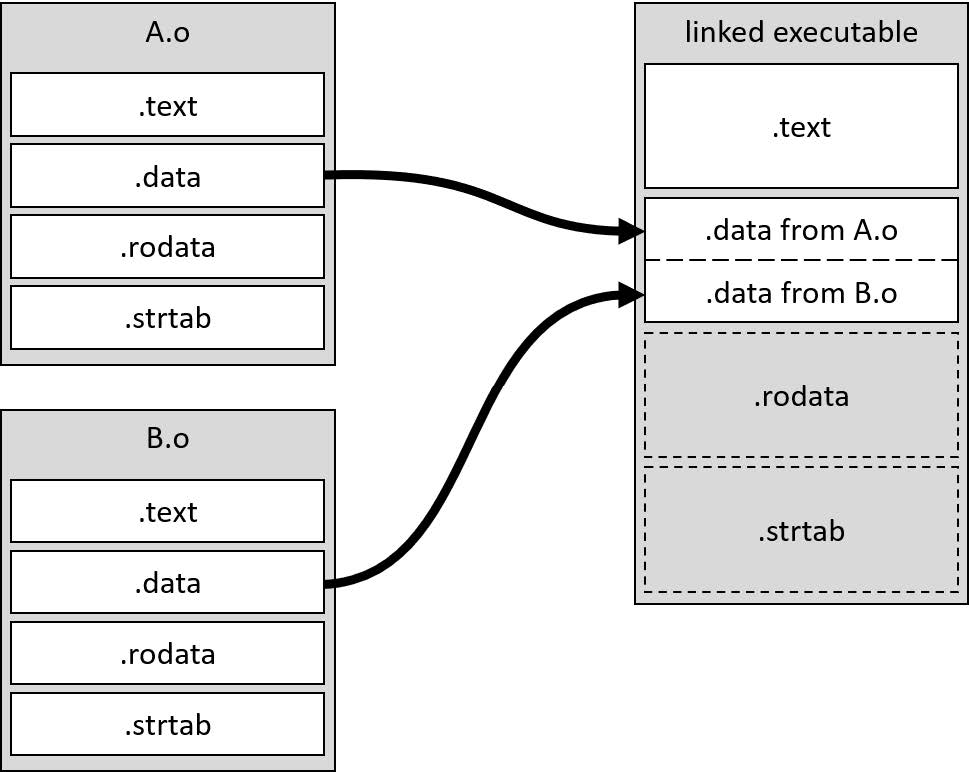
\includegraphics[width=0.8\textwidth]{content/2/chapter6/images/2.jpg}\\
图6.2 .data区段的重定位
\end{center}

其次,链接器需要解析引用。每当来自一个翻译单元的一段代码引用另一个翻译单元中定义的符号时(例如:通过包含其头或使用extern关键字),编译器读取该声明并相信定义就在某个地方,稍后将提供该定义。链接器负责收集这些对外部符号的未解析引用,查找并填充它们在合并到可执行文件后驻留的地址。图6.3显示了一个简单的引用示例:

\begin{center}
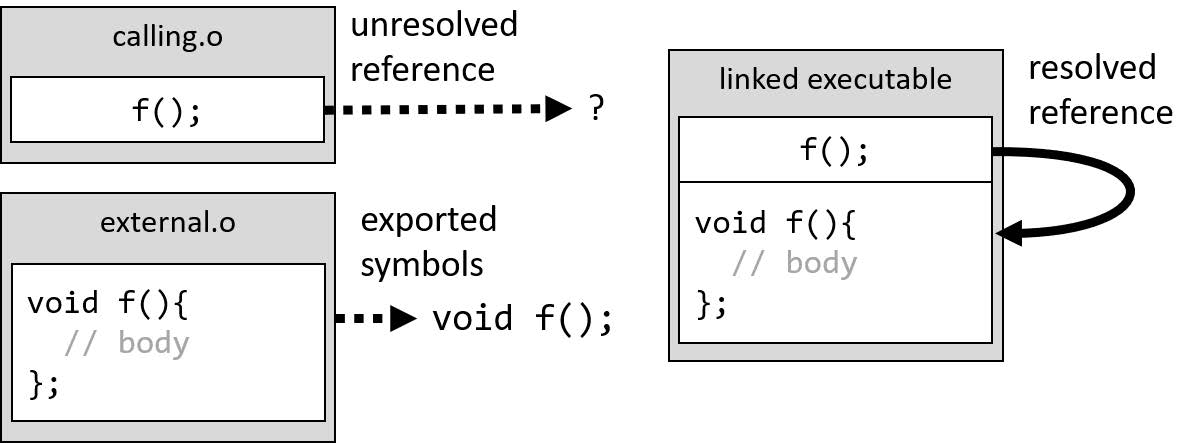
\includegraphics[width=0.8\textwidth]{content/2/chapter6/images/3.jpg}\\
图6.3 一个引用解析
\end{center}

若开发者不知道它是如何工作的,这部分链接可能是问题的来源。我们最终可能会得到无法解析的引用,这些引用找不到外部符号,或者恰恰相反——提供了太多的定义,链接器不知道选择哪一个。

最终的可执行文件看起来非常类似于目标文件,包含带有解析引用的重定位区段、区段头表,当然还有描述整个文件的ELF头。主要的区别是程序头的存在(如图6.4所示)。

\begin{center}
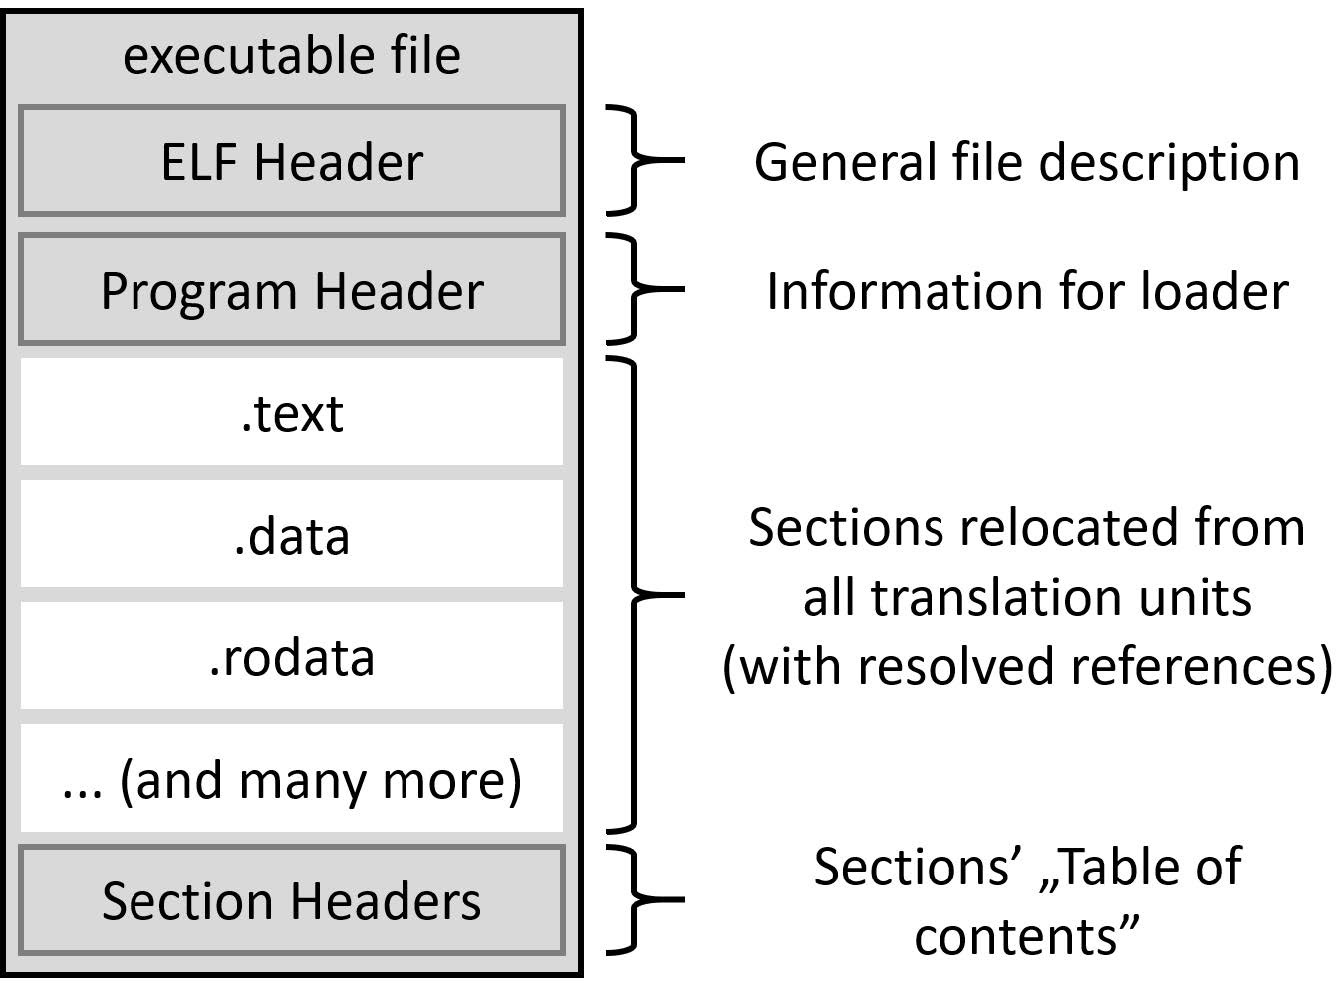
\includegraphics[width=0.8\textwidth]{content/2/chapter6/images/4.jpg}\\
图6.4  ELF中可执行文件的结构
\end{center}

程序头放置在ELF头的右边,系统加载器将读取此头文件以创建进程映像。其头部会包含一些通用信息和内存布局的描述。布局中的每个条目代表一个称为段的内存片段。条目指定将读取哪些节、以什么顺序、虚拟内存中的哪个地址、标志是什么(读、写或执行),以及其他一些有用的细节。

目标文件也可以捆绑在库中,库是一个中间产品,可以在最终的可执行文件或另一个库中使用。下一节中,我们将讨论三种类型的库。



